\section{Performance}

This section discusses preliminary performance of the FEC using physics data production runs from Fall 2018.  This run period used beam energies of 10.6, 7.5 and 6.5 GeV and the CLAS12 Torus magnet polarity set for both inbending and outbending electrons.  The data presented here used the standard FEC FPGA-based electron trigger with a 15 kHz trigger rate and beam currents of 40 nA on a 5~cm LH$_2$ target.

\begin{figure}[hbt]
\centering
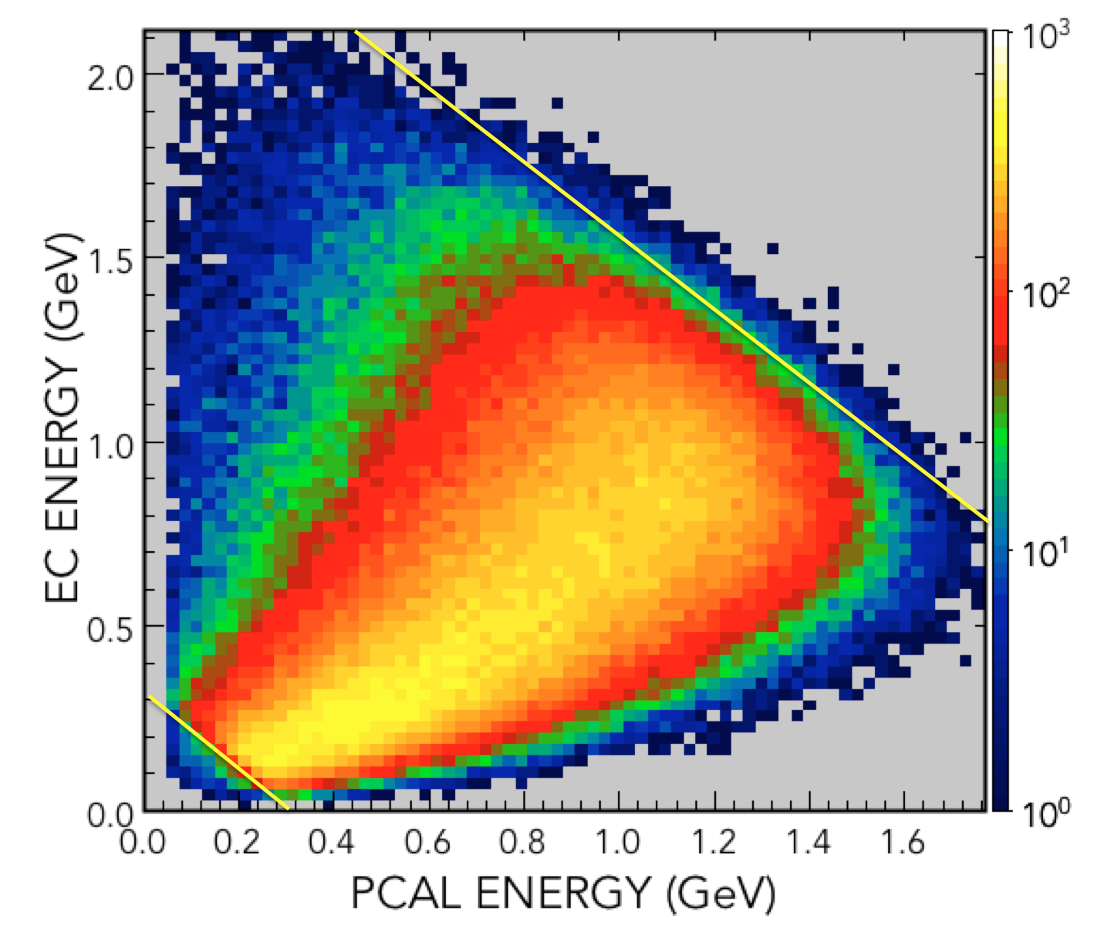
\includegraphics[width=1.0\columnwidth,keepaspectratio]{img/S10_1_000.png}
\caption[]{Reconstructed shower energy in the PCAL and EC modules in response to electrons with a momentum range of 1-10 GeV/c and a polar scattering angle range of 6-34 degrees.  Energies are not corrected for sampling fraction. Diagonal lines show the limits of total reconstructed energy PCAL+EC.}
\label{fig:S10_1_000}
\end{figure}

\subsection{Electron response}
The response of the PCAL and EC components of a single FEC module to high energy electrons is shown in Fig.~\ref{fig:S10_1_000}.  Beam energy was 10.6 GeV and outbending scattered electrons were selected by the Event Builder (EB) service by matching a negative charge DC track to FEC clusters in PCAL, ECIN and ECOU and requiring an activated High Threshold Cerenkov Counter (HTCC) mirror segment that matches the same track.  The plot clearly shows the correlations between energy reconstructed in the forward and rear sections of FEC, while the logarithmic z-scale emphasizes the range of fluctuations. The diagonal lines are total reconstructed  energy with the location of the total energy trigger threshold shown at PCAL+EC = 300 MeV and the other line showing maximum deposited energy consistent with the scattering angle cutoff at $\theta_{elec}=6^o$. Contributions from pions that exceed the 4.7 GeV threshold cutoff of the HTCC were rejected in the hardware trigger using a PCAL energy threshold of 60 MeV, which is also visible in the plot.

The sampling fraction (SF) for electromagnetic showers is defined as the ratio of the total sampled energy (PCAL+EC) to the incident particle energy.  GEANT simulations of electrons impacting the central portion of the FEC show a SF dependence on measured energy ranging from 0.22 to 0.255 over the expected range of electron momentum.  The measured sampling fraction for electrons in the momentum range 1-10 GeV/c is shown in Fig.~\ref{fig:S10_1_0} and follows the expected trend, with some few percent systematic deviations due possibly to residual calibration errors.

\begin{figure}[hbt]
\centering
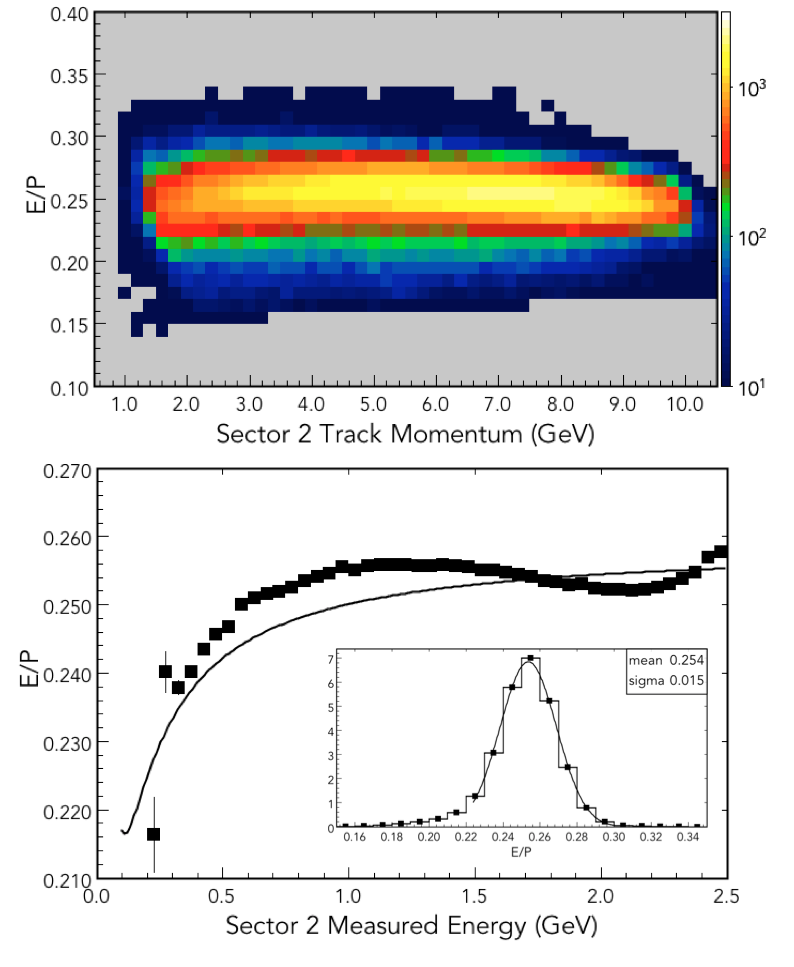
\includegraphics[width=1.0\columnwidth,keepaspectratio]{img/S10_1_0.png}
\caption[]{TOP: Distribution of the ratio E/P of the total measured FEC energy to DC momentum for outbending tracks linked to clusters in PCAL, ECIN and ECOU and identified as electrons by the event builder service.  BOTTOM: E/P versus FEC measured energy compared to GEANT prediction.  Inset shows gaussian fit to overall E/P distribution.}
\label{fig:S10_1_0}
\end{figure}

The variance of the sampling fraction can be expanded as a function of energy with the usual parameterization of contributions \cite{ps1981}:
\begin{equation}
\biggl[\frac{\sigma(E)}{E}\biggr]^2 = \frac{\sigma^2_0}{E^2} + \frac{\sigma^2_1}{E} +\sigma^2_2 + \sigma^2_3 E 
\end{equation}

\begin{itemize}
\item $\sigma_0$ - Pedestal noise, crosstalk.
\item $\sigma_1$ - Poisson statistics (sampling, PMT).
\item $\sigma_2$ - Calibration errors (PMT gains).
\item $\sigma_3$ - Shower leakage fluctuations.
\end{itemize}

Typically $\sigma_0$ is ignored although during MIP based calibration runs the contribution may be non-negligible.  To minimize this contribution all CLAS12 PMT data are taken with fADC pedestals measured and subtracted event-by-event.  Shower leakage contributions to $\sigma_3$ are most important for inbending electrons impacting the FEC at the forwardmost angles, where there is incomplete overlap of PCAL and EC and vanishing acceptance.  

Estimates of the contributions from $\sigma_1$ and $\sigma_2$ were performed using fits to the expected linear dependence of the total relative variance on the inverse of the electron energy as shown in Fig.~\ref{fig:S10_1_1}.  The summary of these fits show an average energy resolution of $9\%/\sqrt{E}$ which is consistent with expectations from GEANT.   The fit results for $\sigma_2$ of around $4\%$ is typical of the present instabilities of PMT gain matching.
 
\begin{figure}[hbt]
\centering
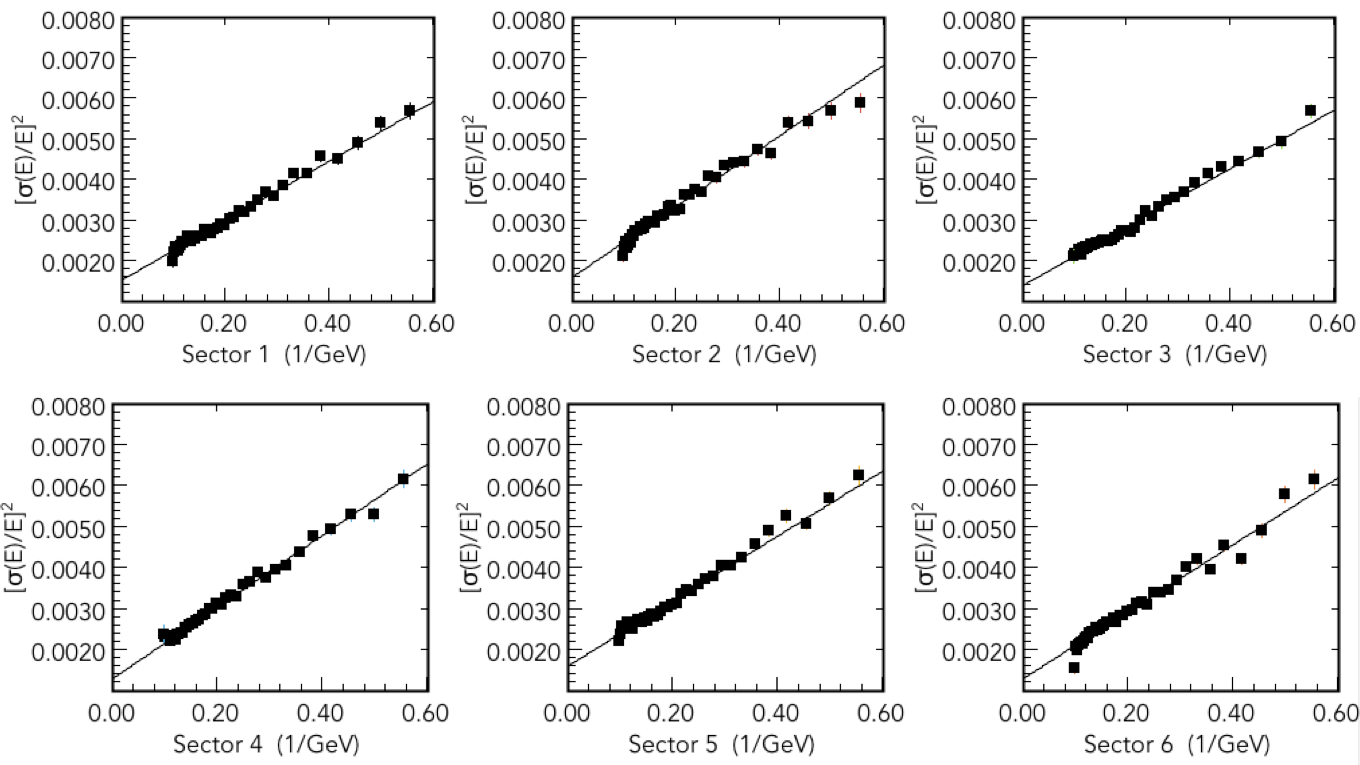
\includegraphics[width=1.0\columnwidth,keepaspectratio]{img/S10_1_1.png}
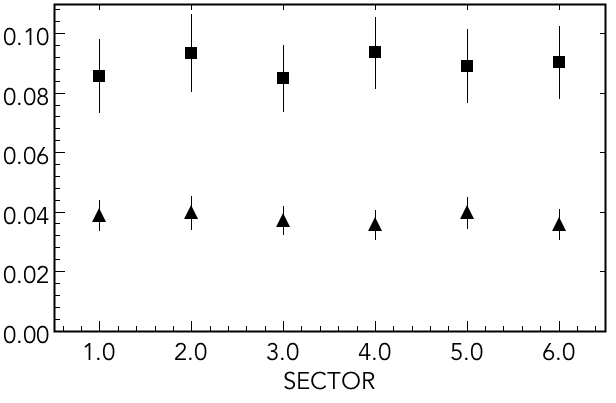
\includegraphics[width=0.5\columnwidth,keepaspectratio]{img/S10_1_2.png}
\caption[]{Relative variance of measured sampling fraction plotted versus inverse of electron energy.  Linear fits used to obtain resolution and calibration variance terms in Eq. 7 are summarized at bottom where $\sigma_1 (\blacksquare)$ and $\sigma_2 (\blacktriangle)$ are plotted versus sector.}
\label{fig:S10_1_1}
\end{figure}

\subsection{Position resolution}
Scintillator alignment and position resolution were estimated from comparison of the reconstructed position of shower clusters with the extrapolation of the DC trajectory state vector of electron tracks from the target to the tracking planes of the PCAL and ECIN.  
Figure~\ref{fig:S10_1_3} summarizes the electron track-cluster matching residuals in the tilted local sector frame.   Systematic offsets of $\approx 1$~cm and $\approx 0.5$ ~cm are seen for PCAL in the radial (perpendicular to the U strips) and transverse (along the direction of the U strips) directions respectively.  These results are consistent with the present uncertainties in scintillator location. The ECIN residuals have not changed from the CLAS era, although the fitted sigmas of the error distributions are smaller, possibly due to the improved angular resolution of the CLAS12 DC tracking and smaller multiple scattering at 10 GeV.  The PCAL residual fits imply an angular resolution of $\approx 0.6$~mrad for showers in the forward detector.  The measured offsets together with survey data will be used to further optimize the track matching cuts used for electron ID and background rejection. 

\begin{figure}[hbt]
\centering
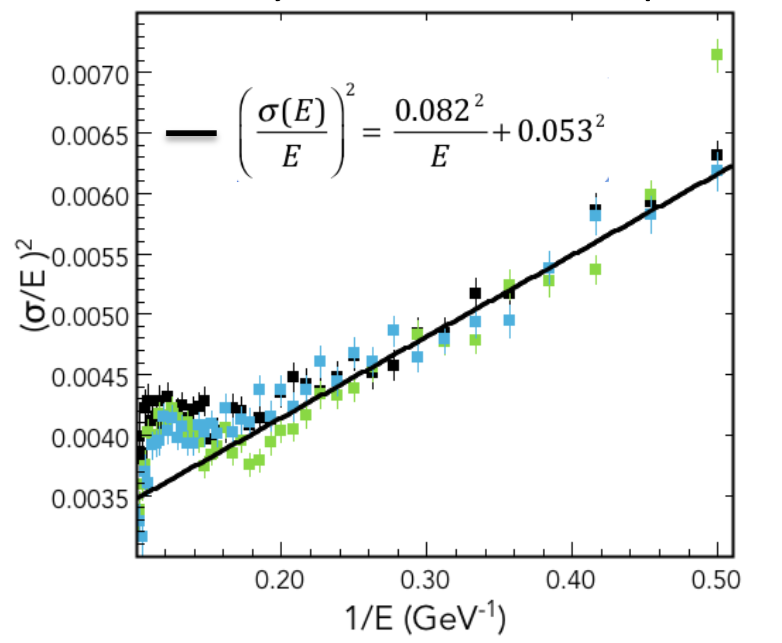
\includegraphics[width=1.0\columnwidth,keepaspectratio]{img/S10_1_3.png}
\caption[]{TOP: Histograms show residual errors in Sector 3 between projected hit position of DC tracks for electrons and reconstructed PCAL cluster position for radial (left) and transverse (right) coordinates. BOTTOM: Sector dependence of radial (black) and transverse (red) residuals for PCAL (left) and ECIN (right).  Errors show sigma of gaussian fits to error distributions.}
\label{fig:S10_1_3}
\end{figure}

\subsection{Reconstruction of $\pi^0\rightarrow 2\gamma$ decays}


\subsection{Neutron detection}
Clusters in the FEC not associated with any reconstructed track in the forward (DC) tracking system are designated neutrals by the event builder service.  Association of neutral PCAL clusters with ECIN and ECOU clusters are based on proximity to straight line trajectories from the CLAS12 origin.  Photons and neutrons are distinguished on the basis of the timing response, with neutrons defined as $\beta < 0.9$.  Experiments which require the exclusive measurement of neutrons in the FEC therefore require both good timing resolution and sufficient detection efficiency. 

Neutron detection in the FEC was measured by tagging neutrons using the $p\,(\,e,e'\,\pi^+\,)\,n$ reaction. Events with missing momentum pointing into the fiducial region of the FEC were selected.  True neutron hits were identified by requiring the direction of the missing momentum to be the same as the direction of a measured neutral cluster within the expected angular resolution, assuming the target center
as origin (Fig.~\ref{S10_4_1}).  

\begin{figure}[hbt]
\centering
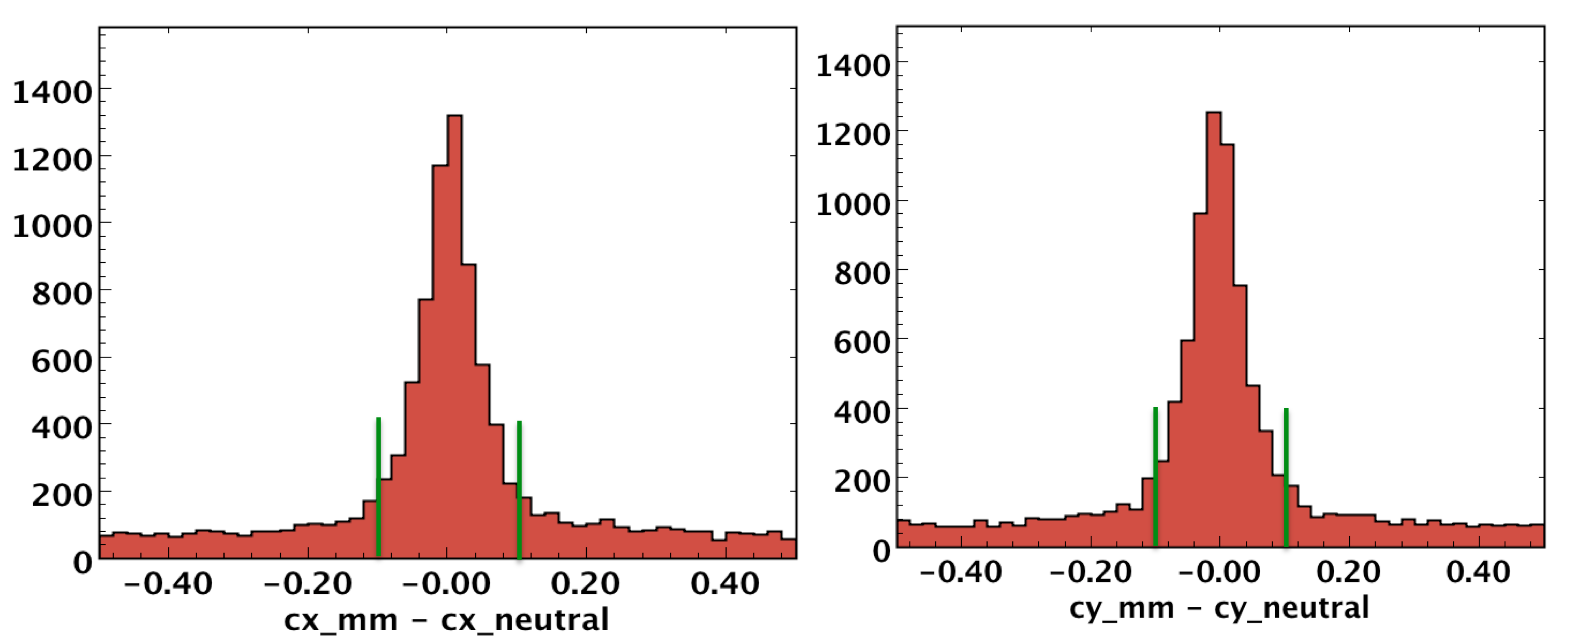
\includegraphics[width=1.0\columnwidth,keepaspectratio]{img/S10_4_1.png}
\caption[]{Differences in $\theta$ and $\phi$ between the detected neutral cluster in the FEC and the missing momentum of the tagged neutron.  The vertical lines indicate cuts used to minimize backgrounds from uncorrelated photons.}
\label{fig:S10_4_1}
\end{figure}

\begin{figure}[hbt]
\centering
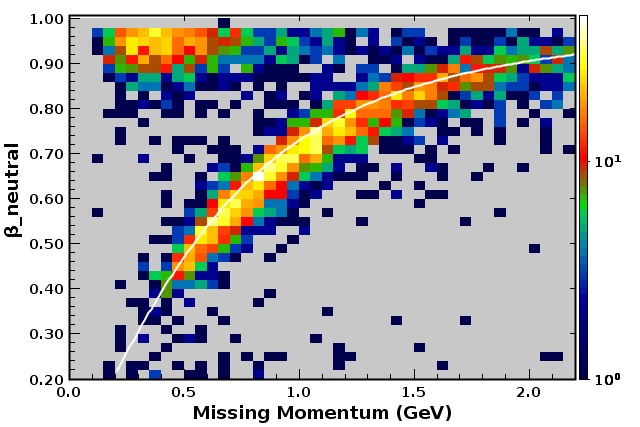
\includegraphics[width=1.0\columnwidth,keepaspectratio]{img/S10_4_2.png}
\caption[]{Correlation between the measured velocity $\beta$ calculated from neutral clusters in the FEC and the missing momentum of the tagged neutron, subject to the $\Delta\theta,\Delta\phi$ cuts shown in Figure 13.  The white line shows the expected correlation from neutrons.}
\label{fig:S10_4_2}
\end{figure}






